\documentclass{beamer}
\mode<presentation>
\usepackage{amsmath}
\usepackage{amssymb}
%\usepackage{advdate}
\usepackage{adjustbox}
\usepackage{subcaption}
\usepackage{enumitem}
\usepackage{multicol}
\usepackage{mathtools}
\usepackage{listings}
\usepackage{url}
\usepackage{tikz}
\usetikzlibrary{matrix, calc}
\def\UrlBreaks{\do\/\do-}
\usetheme{metropolis}
%\usecolortheme{lily}
\setbeamertemplate{footline}
{
	\leavevmode%
	\hbox{%
		\begin{beamercolorbox}[wd=\paperwidth,ht=2.25ex,dp=1ex,right]{author in head/foot}%
			\insertframenumber{} / \inserttotalframenumber\hspace*{2ex} 
		\end{beamercolorbox}}%
		\vskip0pt%
	}
	\setbeamertemplate{navigation symbols}{}

	\providecommand{\nCr}[2]{\,^{#1}C_{#2}} % nCr
	\providecommand{\nPr}[2]{\,^{#1}P_{#2}} % nPr
	\providecommand{\mbf}{\mathbf}
	\providecommand{\pr}[1]{\ensuremath{\Pr\left(#1\right)}}
	\providecommand{\qfunc}[1]{\ensuremath{Q\left(#1\right)}}
	\providecommand{\sbrak}[1]{\ensuremath{{}\left[#1\right]}}
	\providecommand{\lsbrak}[1]{\ensuremath{{}\left[#1\right.}}
	\providecommand{\rsbrak}[1]{\ensuremath{{}\left.#1\right]}}
	\providecommand{\brak}[1]{\ensuremath{\left(#1\right)}}
	\providecommand{\lbrak}[1]{\ensuremath{\left(#1\right.}}
	\providecommand{\rbrak}[1]{\ensuremath{\left.#1\right)}}
	\providecommand{\cbrak}[1]{\ensuremath{\left\{#1\right\}}}
	\providecommand{\lcbrak}[1]{\ensuremath{\left\{#1\right.}}
	\providecommand{\rcbrak}[1]{\ensuremath{\left.#1\right\}}}
	\theoremstyle{remark}
	\newtheorem{rem}{Remark}
	\newcommand{\sgn}{\mathop{\mathrm{sgn}}}
	\providecommand{\abs}[1]{\left\vert#1\right\vert}
	\providecommand{\res}[1]{\Res\displaylimits_{#1}} 
	\providecommand{\norm}[1]{\lVert#1\rVert}
	\providecommand{\mtx}[1]{\mathbf{#1}}
	\providecommand{\mean}[1]{E\left[ #1 \right]}
	\providecommand{\fourier}{\overset{\mathcal{F}}{ \rightleftharpoons}}
	%\providecommand{\hilbert}{\overset{\mathcal{H}}{ \rightleftharpoons}}
	\providecommand{\system}{\overset{\mathcal{H}}{ \longleftrightarrow}}
	%\newcommand{\solution}[2]{\textbf{Solution:}{#1}}
	%\newcommand{\solution}{\noindent \textbf{Solution: }}
	\providecommand{\dec}[2]{\ensuremath{\overset{#1}{\underset{#2}{\gtrless}}}}
	\newcommand{\myvec}[1]{\ensuremath{\begin{pmatrix}#1\end{pmatrix}}}
		\let\vec\mathbf

		\lstset{
			%language=C,
			frame=single, 
			breaklines=true,
			columns=fullflexible
		}

		\numberwithin{equation}{section}

		\title{Sprog Presentation}
		\author{Akshara Sarma Chennubhatla,\\ EE24BTECH11003,\\IIT Hyderabad.\\}

		\date{\today} 
		\begin{document}

		\begin{frame}
			\titlepage
		\end{frame}

		\begin{frame}
			\frametitle{Problem Statement}
Solve the following pair of linear equations,
\begin{align}
	\sqrt{2}x + \sqrt{3}y &= 0\\
	\sqrt{3}x - \sqrt{8}y &= 0
\end{align}
\end{frame}
\subsection{Solution}
\begin{frame}
      \frametitle{Solution-1}
	Let
\begin{align}
	\vec{x} = \myvec{x\\y}
\end{align}
Expressing the system in matrix form,
\begin{align}
	\myvec{\sqrt{2} & \sqrt{3} \\ \sqrt{3} & -\sqrt{8}}\vec{x} &= \myvec{0 \\ 0}\\
	\text{which is of the form } A\vec{x} &= \vec{0}
\end{align}
Any non-singular matrix $A$ can be expressed as a product of an upper triangular matrix $U$ and a lower triangular matrix $L$, such that
\begin{align}
	A &= LU\\
	\implies LU\vec{x} &= \vec{0}
\end{align}

\end{frame}
\begin{frame}
	\frametitle{Solution-1}
	$U$ is determined by row reducing $A$ using a pivot,
\begin{align}
	\myvec{\sqrt{2} & \sqrt{3}\\\sqrt{3} & -\sqrt{8}} \xrightarrow {R_2 \to R_2 - \sqrt{\frac{3}{2}}R_1} \myvec{\sqrt{2} & \sqrt{3}\\0 & -\sqrt{8} - \frac{3}{2}}
\end{align}
Let 
\begin{align}
	L = \myvec{1 & 0\\l & 1}
\end{align}
$l$ is the multiplier used to zero out $a_{21}$ in $A$.
\begin{align}
	L = \myvec{1 & 0 \\ \sqrt{\frac{3}{2}} & 1}
\end{align}
\end{frame}
\begin{frame}
	\frametitle{Solution-2}
	This $LU$ decomposition could also be computationally found using Doolittle's algorithm. The update equation is given by,
\begin{align}
	U_{ij} &= \begin{cases}
		A_{ij} & \quad i = 0\\
		A_{ij} - \sum_{k = 0}^{i - 1} L_{ik} U_{kj} & \quad i > 0
	\end{cases}\\
	L_{ij} &= \begin{cases}
		\frac{A_{ij}}{U_{jj}} & \quad j = 0, U_{jj} \neq 0\\
		\frac{A_{ij} - \sum_{k = 0}^{j - 1} L_{ik} U_{kj}}{U_{jj}} & \quad j > 0
	\end{cases}
\end{align}
\end{frame}
\begin{frame}
	\frametitle{Solution-2}
	Let $\vec{y} = U\vec{x}$,
\begin{align}
	L\vec{y} = \vec{0}
\end{align}
After we find $\vec{y}$, we find $\vec{x}$ using the following equation,
\begin{align}
	U\vec{x} = \vec{y}
\end{align}
Applying forward substitution on the equation, we get,
\begin{align}
	\myvec{1 & 0\\\sqrt{\frac{3}{2}} & 1}\myvec{y_1\\y_2} &= \myvec{0\\0}\\
	y_1 &= 0\\
	\sqrt{\frac{3}{2}}y_1 + y_2 &= 0\\
	\implies \myvec{y_1\\y_2} &= \myvec{0\\0}
\end{align}
\end{frame}
\begin{frame}
	\frametitle{Solution-2}
	Substituting $\vec{y}$ in the equation, we get,
\begin{align}
	\myvec{\sqrt{2} & \sqrt{3}\\0 & -\sqrt{8} - \frac{3}{2}} \myvec{x\\y} &= \myvec{0\\0}\\
	\sqrt{2}x + \sqrt{3}y &= 0\\
	\brak{-\sqrt{8} - \frac{3}{2}}y &= 0\\
	\implies x &= 0, y = 0\\
	\implies \myvec{x\\y} &= \myvec{0\\0}
\end{align}
This shows that the pair of linear equations have exactly one solution.
\end{frame}
\begin{frame}
	\frametitle{Result}
	Below is the $LU$ decomposition of this matrix got through the c code.

L:\\
1.000000  0.000000\\
1.224745  1.000000\\
U:\\
1.414214 1.732051\\
0.000000 -4.949748

\end{frame}
\begin{frame}
	\frametitle{Plot}
	Below is the plot of the pair of lines representing the linear equations and their point of intersection.
\begin{figure}[h!]
	\centering
	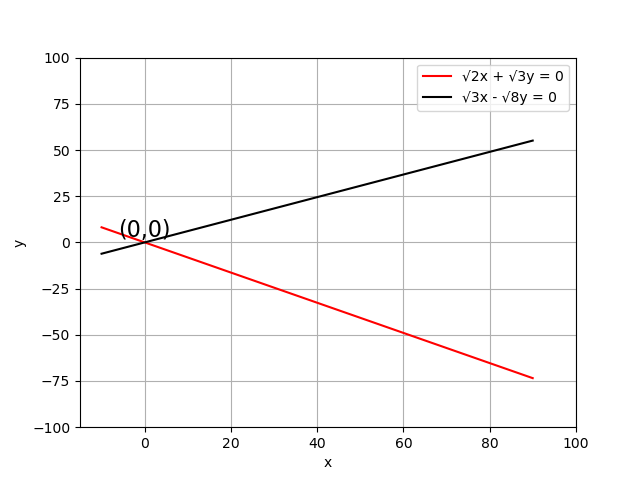
\includegraphics[width=0.6\columnwidth]{figs/simulated.png}
	\caption{Plot of the linear equations and their intersection point}
	\label{label}
\end{figure}
\end{frame}
\end{document}
